
%%%%%%%%%%%%%%%%%%%%%%
\subsection{Dark Matter relic density and direct/indirect detection}

The results from PLANCK~\cite{Ade:2013zuv,Planck:2015xua} (see also WMAP~\cite{Hinshaw:2012aka}) have further decreased the error on the already quite precise measurement of the dark matter relic density, $\Omega_{\rm DM} h^2$:
\begin{equation}
\Omega_{\rm DM}^{\rm Planck} h^2=0.1184\pm0.0012.
\label{eq:planck-limit}
\end{equation} 
In the i2HDM model, the lightest inert scalar $h_1$ is stable and contributes to this relic density.
In our study we take the upper limit on  $\Omega_{\rm DM} h^2$ as the hard one,
excluding the parameter space points which lead to DM overabundance.
However we do not exclude the i2HDM parameter space regions where $h_1$ is under-abundant,
allowing for other sources of DM coming from an additional new physics sector.

We have evaluated $\Omega_{\rm DM} h^2$ with the
{\texttt{micrOMEGAs 2.4.1}} package~\cite{Belanger:2013oya,Belanger:2006is, Belanger:2010gh}
since it directly reads the model files in CalcHEP format.
Fig.~\ref{fig:1d-mh1-Omega}(a) shows the relic density in the case of quasi-degenerate $h_1,h_2$ and $h^+$ masses, 
$M_{h_2}=M_{h^+}=M_{h_1}+\Delta M= M_{h_1}+$1~GeV.
This case is qualitatively different from the case with a non-negligible mass splitting
as illustrated in Fig.~\ref{fig:1d-mh1-Omega}(b), where we chose  $M_{h_2}=M_{h^+}=M_{h_1}+\Delta M=M_{h_1}+$100~GeV.
One should also note that scenarios with positive or negative $\lambda_{345}$ values of the same magnitude
are qualitatively similar, except for the effect of interference (see dashed versus solid curves in Fig.~\ref{fig:1d-mh1-Omega}). 
One can observe the following effects and features of the model in Fig.~\ref{fig:1d-mh1-Omega}:
\begin{itemize}
\item The red-shaded region in Fig.~\ref{fig:1d-mh1-Omega}(a) 
is excluded by the LEP data, since in this region $W$ and $Z$ bosons would decay to the light inert scalars. 
Respectively, the effect of the resonant co-annihilation, $h_1 h_2 \to Z$ and $h_1 h^+ \to W^+$, can be seen 
in this region in the first two dips for $M_{h_1} \sim 40$ and $45$~GeV.
These processes are governed by the gauge coupling constant and are independent of $\lambda_{345}$. 
\item
In the case of larger $M_{h_2}-M_{h_1}$  mass split (Fig.~\ref{fig:1d-mh1-Omega}(b)), 
this effect disappears since $M_{h_1}+M_{h_2} > M_Z$ and $M_{h_1}+M_{h^+} > M_W$.
\item
The sharpest dip in the $\Omega_{\rm DM} h^2$ dependence of $M_{h_1}$ is at 65 GeV and 
corresponds to the DM annihilation through the Higgs boson $h_1 h_1 \to H$. It is present in both cases. 
\item
At higher masses, we observe a wider and more shallow  dip at around 80-90 GeV from  $h_1
h_1\to W^+W^-$ and $h_1 h_1\to ZZ$ channels which are merged together. 
\item
Finally, the last dip around 125 GeV corresponds to the
reduction of the DM relic density  due to the opening of the $ h_1 h_1\to HH$ annihilation channel. This dip takes place only for 
large values of $\lambda_{345}$, which provide a high enough rate for the $h_1h_1\to HH$ process via the $s$-channel Higgs boson. 
\item
The pattern of these last three dips is the same for the larger mass split scenario presented in Fig.~\ref{fig:1d-mh1-Omega}(b). 
In both scenarios, the interference effect is sensitive to the sign of $\lambda_{345}$ and appears in this region 
as a result of the positive or negative interference of the $s$-channel Higgs boson exchange
diagram and the rest of annihilation diagrams.
\item
One can also observe qualitative differences in the asymptotic behaviour of the DM relic density for small
and large $M_{h_1}$ values for different $\Delta M$. In the $\Delta M=1$~GeV case with $M_{h_1} < 65$~GeV, the effective
co-annihilation of the inert scalars keeps the DM density always below the PLANCK limit. 
For $\Delta M=100 $~GeV, DM co-annihilation is suppressed and the relic density  is equal or below the experimental
limit only for large values of $\lambda_{345}$ ($\lambda_{345} \gtrsim 0.3$) which are excluded by LHC
limits on the invisible Higgs decay, see Eq.~(\ref{lam345-limit-from-inv}).
\item
For $M_{h_1}$ well above 65 GeV, co-annihilation effects become less important
in comparison with $h_1 h_1$ annihilation into vector bosons,
which opens in this region.
For this annihilation process the quartic couplings of DM with longitudinal vector bosons $h_1h_1 V_L V_L$ play an important role. 
For $h_1 h_1 Z_L Z_L$, it is equal to $\tilde\lambda_{345}$ defined in (\ref{tildelam345}), while for
$h_1 h_1 W_L W_L$ it is given by $\lambda_3 = \lambda_{345} + 2(M_{h^+}^2-M_{h_1}^2)/v^2$.
For small mass splittings $\Delta M_c = M_{h^+}-M_{h_1}$ and $\Delta M_2 = M_{h_2}-M_{h_1}$, 
the correspondingly small values of the $h_1h_1 V_L V_L$ quartic couplings 
generate a low $h_1 h_1$ annihilation cross section $\braket{\sigma v}$, which decreases with growing $M_{h_1}$.
Eventually this leads to comparatively high value of $\Omega_{\rm DM} h^2$
(which increases with $M_{h_1}$ both
due to the decrease of $\braket{\sigma v}$ as well as the increase of the DM mass)
which  reaches  the PLANCK limit for large enough $M_{h_1}$ 
as one can see from  Fig.~\ref{fig:1d-mh1-Omega}(a).
On the contrary, for large $\Delta M_c$ and/or $\Delta M_2$, the mass splittings generate
a high rate for $h_1 h_1$ annihilation into vector bosons, which rises with growing $M_{h_1}$. 
This generates a DM density below the experimental limit even for large values of $M_{h_1}$.
In this scenario the potential increase of  $\Omega_{\rm DM} h^2$ due the large DM mass
is compensated by the respective increase of  $\braket{\sigma v}$
and leads to an approximately flat $\Omega_{\rm DM} h^2$ versus $M_{h_1}$
in the 100--1000 GeV  range.
This makes the asymptotic behaviour of the DM density versus $M_{h_1}$ qualitatively different for $\Delta M = 100$ GeV 
as compared to $\Delta M = 1$ GeV, see Fig.~\ref{fig:1d-mh1-Omega}(b).
These two scenarios with the large and small $\Delta M_c$, $\Delta M_2$ mass splittings 
qualitatively cover the whole parameter space of the i2HDM.
\end{itemize} 

\begin{figure}[htb]
\centering
{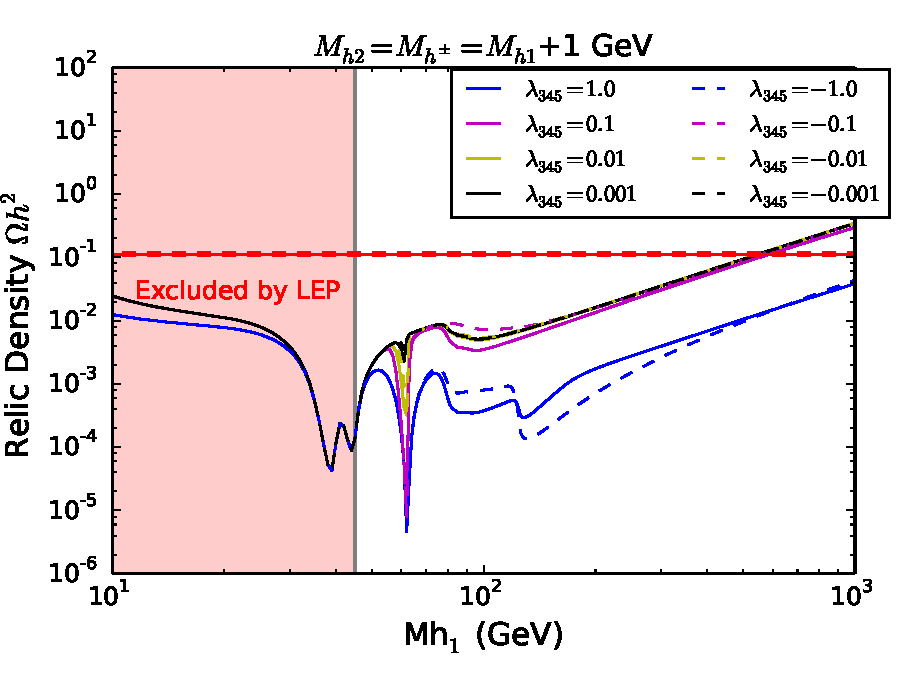
\includegraphics[width=0.5\textwidth]{Figures/Omega_Mh1_new.pdf}}%
{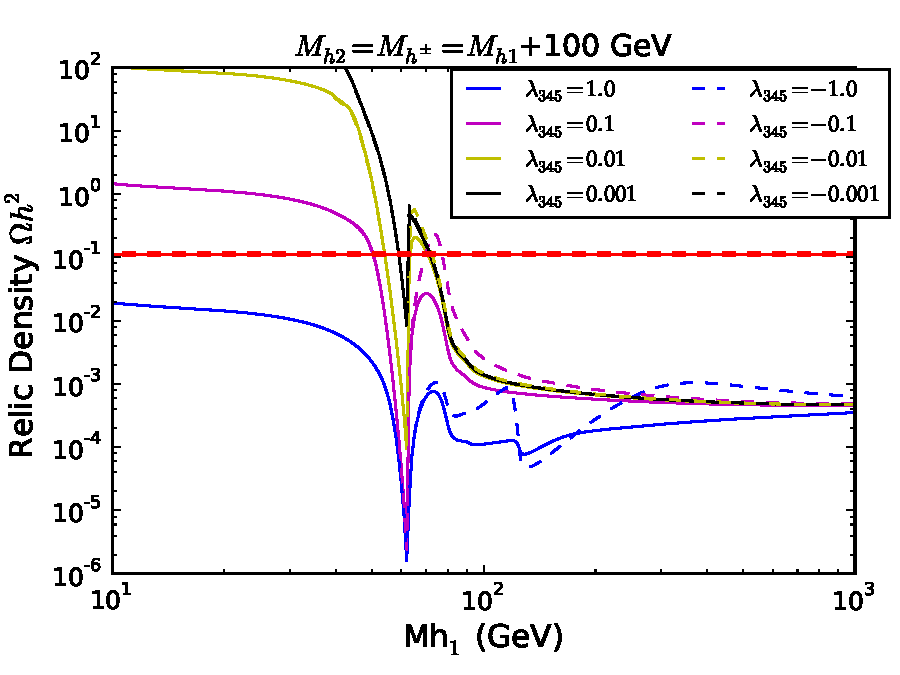
\includegraphics[width=0.5\textwidth]{Figures/Omega_Mh1_mh+100_new.pdf}}%
\vskip -0.5cm\hspace*{-3cm}(a)\hspace*{0.48\textwidth}(b)
\caption{The relic density, $\Omega_{\rm DM} h^2$,   as a function of $M_{h_1}$
for various $\lambda_{345}$ parameters. The red-shaded region in the left frame is excluded by the LEP data, 
since in this region $W$ and $Z$ bosons would decay to the light inert scalars. 
The horizontal red line corresponds to the relic density upper limit given by Eq.(\ref{eq:planck-limit}).}
\label{fig:1d-mh1-Omega}
\end{figure}
%
 
 
\begin{figure}[htb]
\centering
{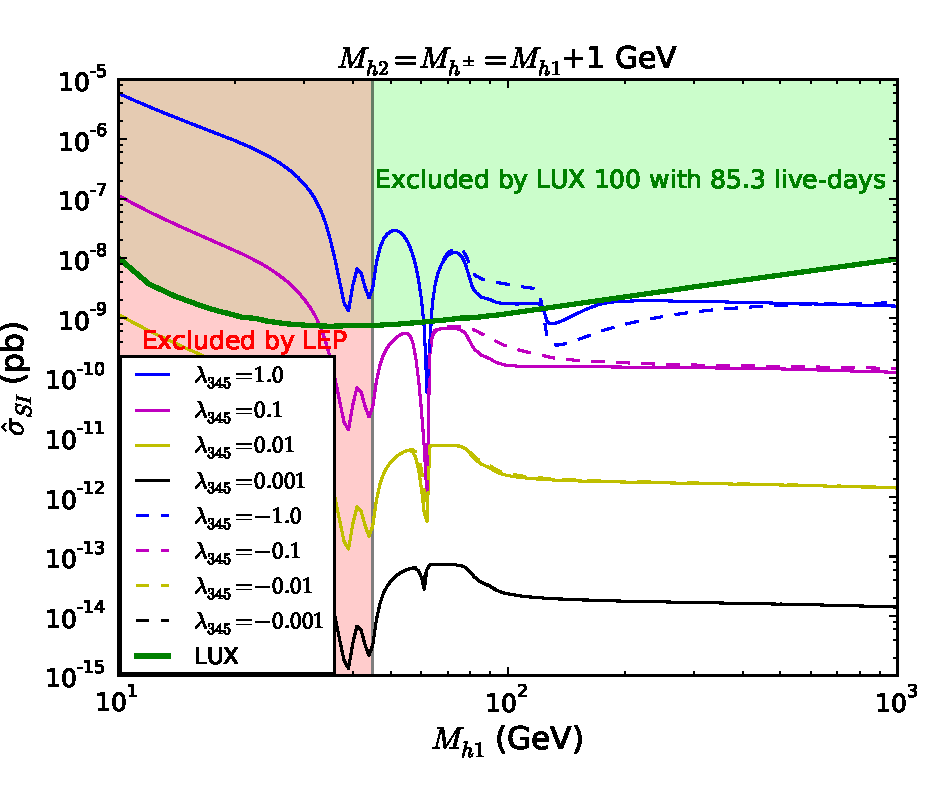
\includegraphics[width=0.5\textwidth]{Figures/DD_LUX_limit_new.pdf}}%
{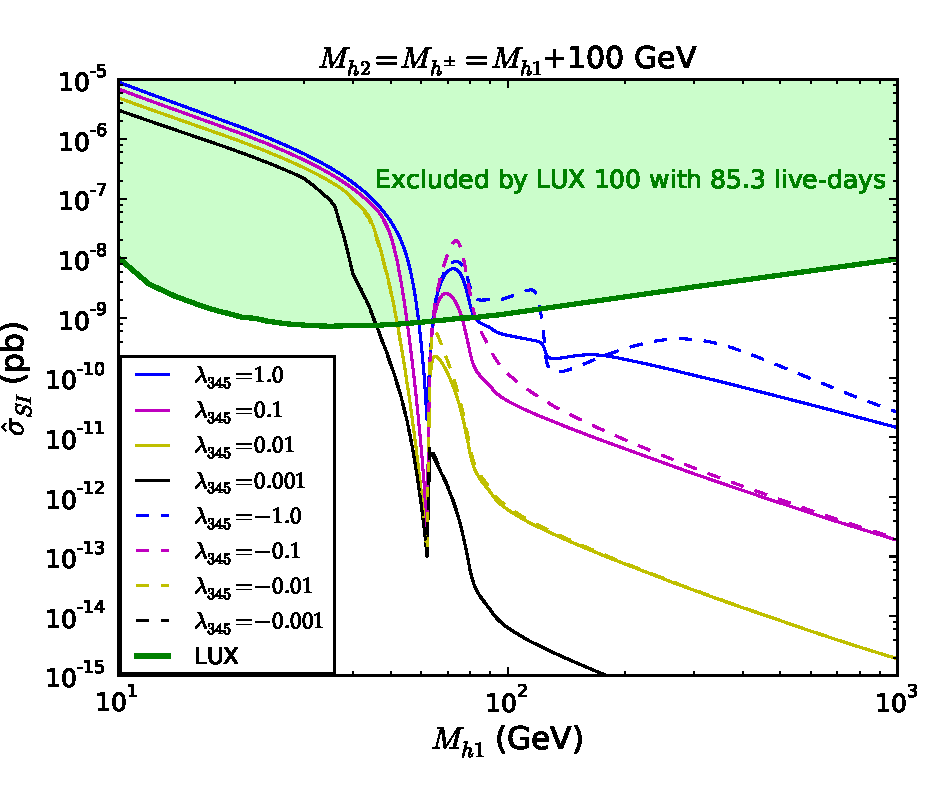
\includegraphics[width=0.5\textwidth]{Figures/DD_LUX_limit_mh+100_new.pdf}}%
\vskip -0.5cm\hspace*{-3cm}(a)\hspace*{0.48\textwidth}(b)
\caption{Rescaled spin independent direct detection rates $\hat{\sigma}_{SI}$ versus $M_{h_1}$ and the LUX100 constraint.
 The red-shaded region in the left frame is excluded by LEP data.
\label{fig:1d-mh1-DD}}
\end{figure}



We have also checked whether the i2HDM parameter space is consistent with the limits from  DM direct detection (DD) experiments.
We have evaluated the spin-independent cross section of DM scattering off the proton, $\sigma_{SI}$,
 also using the \texttt{micrOMEGAs} package.
In Fig.~\ref{fig:1d-mh1-DD} limits from LUX100 are shown by the shaded green area where the left and right frames
illustrate the small and large $\Delta M$  scenarios as in Fig.~\ref{fig:1d-mh1-Omega}.
To present the results in Fig.~\ref{fig:1d-mh1-DD}, we use the re-scaled DD cross section, $\hat{\sigma}_{SI}= 
R_\Omega\times \sigma_{SI}$, where the scaling factor
$R_\Omega = \Omega_{\rm DM}/\Omega^{\rm Planck}_{\rm DM}$ takes into account the case of $h_1$
representing only a part of the total DM budget, thus allowing for a convenient comparison
of the model prediction with the limits from LUX \cite{Akerib:2013tjd}.

The flat asymptotic of $\hat{\sigma}_{SI}$ in Fig.~\ref{fig:1d-mh1-DD}(a)
for high $M_{h_1}$ means that the decrease of the 
proton-DM scattering cross section ${\sigma}_{SI}$ with increasing $M_{h_1}$ is compensated by the 
growth of the relic density which one can observe in Fig.~\ref{fig:1d-mh1-Omega}(a).
{In Fig.~\ref{fig:1d-mh1-DD}(b), on the other hand, $\hat{\sigma}_{SI}$
drops with large and increasing values of $M_{h_1}$.
This can be understood by observing from Fig.~\ref{fig:1d-mh1-Omega}(b) that in this region
$R_\Omega = \Omega_{\rm DM}/\Omega^{\rm Planck}_{\rm DM}\simeq$ constant, and therefore 
the asymptotic behaviour of $\hat{\sigma}_{SI}$ is the same as for ${\sigma}_{SI}$,
that is, it goes down as $M_{h_1}$ grows due to the reduced $\braket{\sigma v}$.}



%\giac{[COMMENT:}{ we need to add a reference to LUX results. Are there other references studying this constraint?]}

A related question is whether the model can be better probed by   indirect detection (ID) experiments, i.e. the detection of   energetic cosmic rays like $e^+$, $\gamma$, $p$ or $\bar{p}$, which may be created by the annihilation of $h_1$ pairs.
We have checked  that the strongest bounds on the i2HDM parameter space
 coming from such experiments are set by gamma ray telescopes: both the Fermi-LAT gamma-ray space telescope~\cite{Ackermann:2011wa} as well as ground based telescopes. Fermi-LAT is sensitive to gamma rays particularly in the low mass range  up to $\mathcal{O}(100\,\mathrm{GeV})$, but the bounds are not competitive with those coming from DD. 
This conclusion is also confirmed by studies in Ref.~\cite{Arhrib:2013ela}.
%\giac{[COMMENT:}{ add references on this conclusion on ID vs. DD]}
 

